\documentclass[border=10pt]{standalone}

\usepackage{tikz}
\usepackage{tikzsymbols}
\usetikzlibrary{calc,patterns,shapes.geometric}

\def\centerarc[#1](#2)(#3:#4:#5){\draw[#1] ($(#2)+({#5*cos(#3)},{#5*sin(#3)})$) arc (#3:#4:#5);}

\begin{document}
	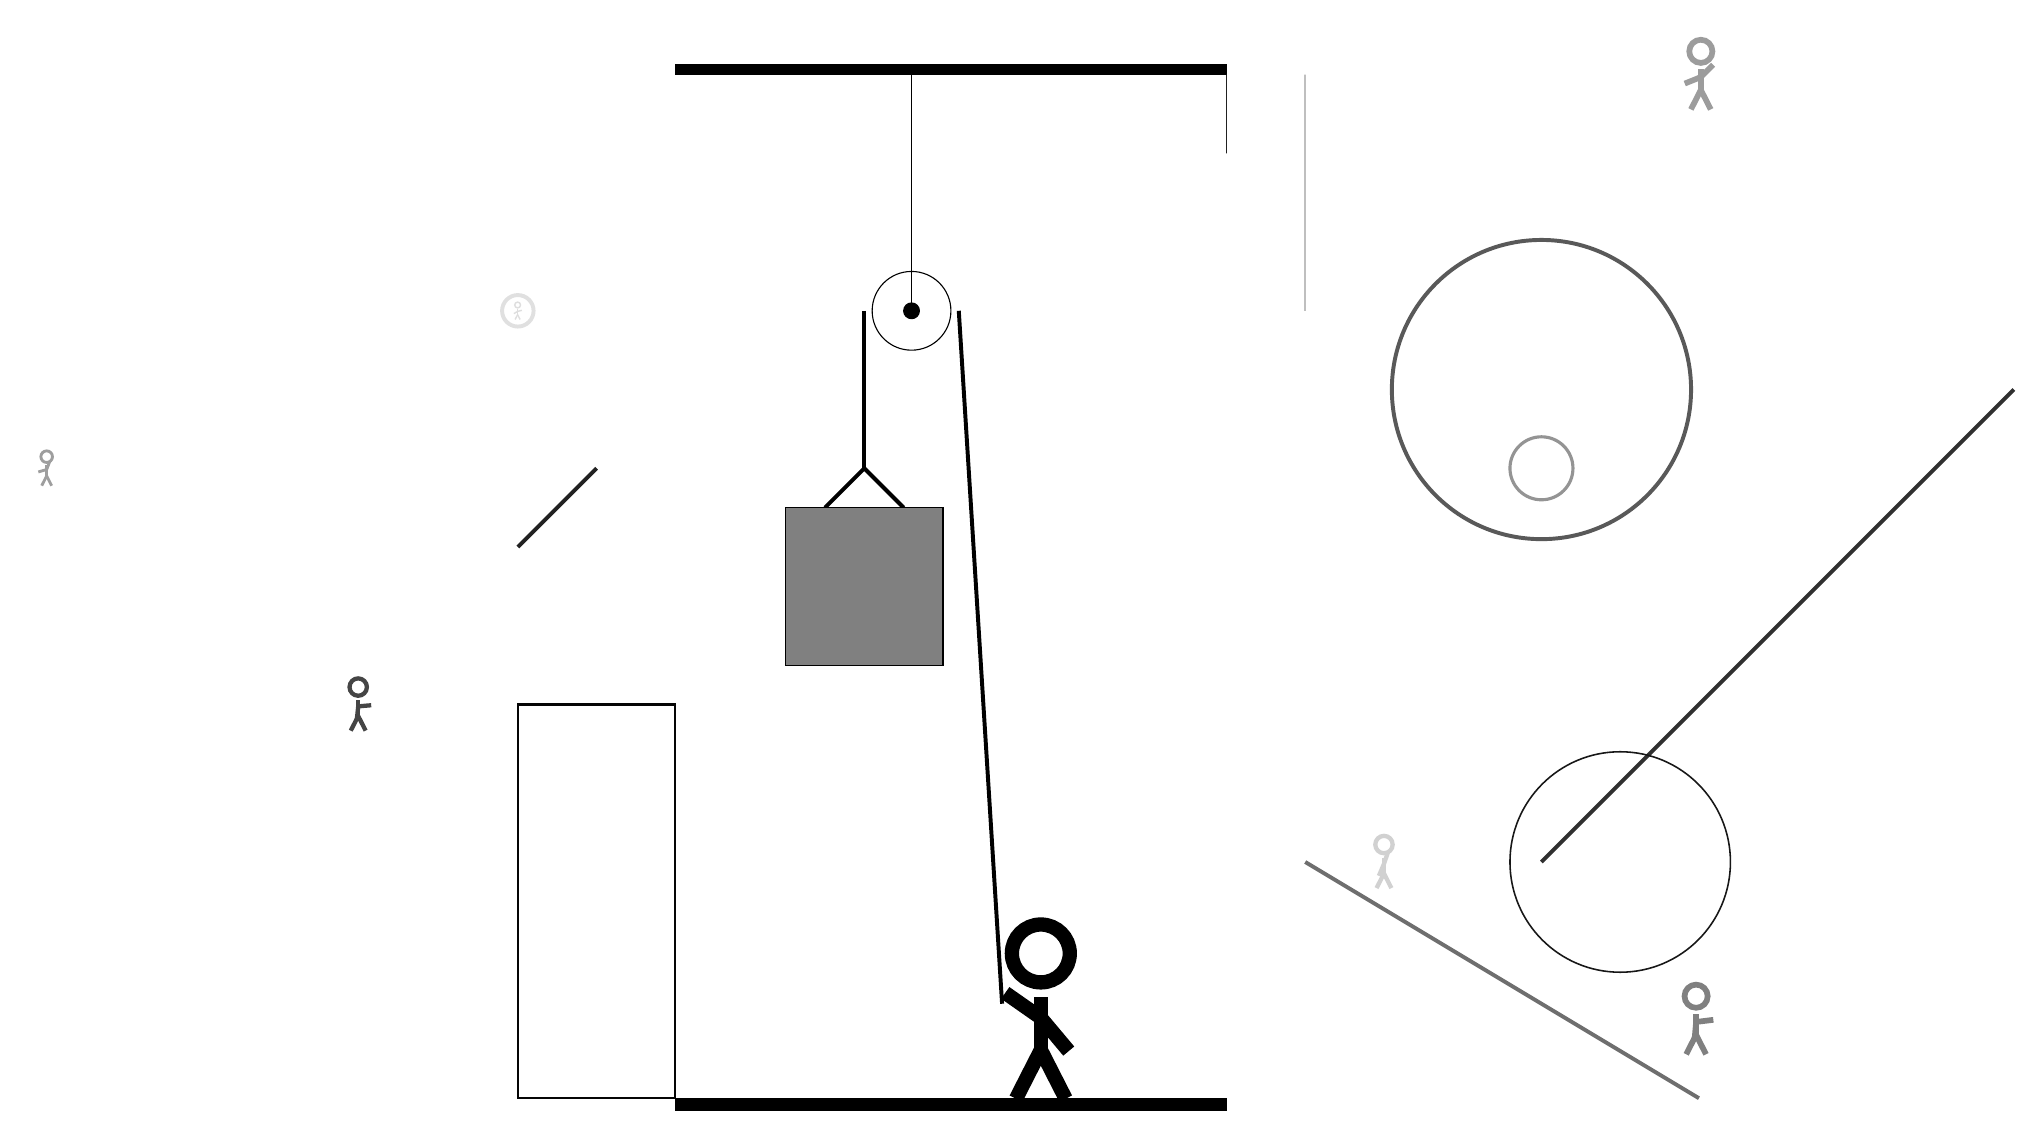
\begin{tikzpicture}
		%%%%% START %%%%%
		
		\draw[fill=black] (-2, 10) rectangle (5, 10.125);
		
		\draw (1, 7) circle (0.5);
		\draw[fill=black] (1, 7) circle (0.1);
		\draw (1, 10) -- (1, 7);
		
		\draw[line width=0.5mm] (-0.1, 4.5) -- (0.4, 5.0) -- (0.9, 4.5);
		\draw[fill=black!50] (-0.6, 4.5) rectangle (1.4, 2.5);
		
		\draw[line width=0.5mm] (0.4, 7) -- (0.4, 5.0);
		\centerarc[line width=0.5mm](1, 7)(0:180:0.6);
		\draw[line width=0.5mm](1.6, 7) -- (2.15, -1.8);
		
		\draw[line width=0.5mm, color=black!81](9, 0) -- (15, 6);
		
		\draw [line width=0.2mm, color=black!91](10, 0) circle (1.4);
		\node[line width=0.3mm, color=black!39] at (11, 10) {\Strichmaxerl[4][22][45]};
		\draw[line width=0.3mm, color=black!98] (-2, -3) rectangle (-4, 2);
		\node[line width=0.4mm, color=black!18] at (7, 0) {\Strichmaxerl[3][67][71]};
		\draw[line width=0.5mm, color=black!87](-3, 5) -- (-4, 4);
		\draw [line width=0.4mm, color=black!42](9, 5) circle (0.4);
		\node[line width=0.7mm, color=black!13] at (-4, 7) {\Strichmaxerl[1][30][15]};
		\draw [line width=0.5mm, color=black!65](9, 6) circle (1.9);
		\node[line width=0.3mm, color=black!73] at (-6, 2) {\Strichmaxerl[3][84][5]};
		\node[line width=0.7mm, color=black!38] at (-10, 5) {\Strichmaxerl[2][16][69]};
		\draw[line width=0.5mm, color=black!57](6, 0) -- (11, -3);
		\node[line width=0.6mm, color=black!50] at (11, -2) {\Strichmaxerl[4][85][7]};
		
		\draw[line width=0.2mm, color=black!87] (5, 10) rectangle (5, 9);
		\draw [line width=0.5mm, color=black!12](-4, 7) circle (0.2);
		\draw[line width=0.2mm, color=black!25] (6, 10) rectangle (6, 7);
		
		\node at (2.6, -1.9) {\Strichmaxerl[10][-35][-50]};
		
		\draw[fill=black] (-2, -3) rectangle (5, -3.15);
		
		%%%%% END %%%%%
	\end{tikzpicture}
\end{document}